\documentclass[11pt]{article}

%What I'm running to compile the mo': make veryclean; make pdf; make ; gnome-open paper.pdf
%Dependencies on ubuntu: sudo aptitude install biblatex-dw biblatex gedit-latex-plugin

% This should fix widow and orphan paragraphs, I think [mlissner]
\clubpenalty = 10000
\widowpenalty = 10000

% Make our citation numbers superscript. No longer necessary with biblatex code below. [mlissner]
%\usepackage{overcite}

% Make pdf bookmarks for the mo'. Make them NOT have a crazy red border. [mlissner]
\usepackage[bookmarks=true, pdfborder = 0]{hyperref}

% Make images work
\usepackage[pdftex]{graphicx}


% Do citations as footnotes.
\usepackage[style=footnote-dw]{biblatex}
\bibliography{bibliography}

\begin{document}

% this title is meh, but sort of works. Might be stronger words than we intend. Might not be.
\title{CourtListener.com: A platform for researching and staying abreast of the latest in the law}

% in alphabetical order, by last name
\author{Michael Lissner, advised by, and with much debt to Brian Carver}
\date{May 7, 2010}
\maketitle
\begin{quote}
``Such an undertaking is not only possessed of great intrinsic merit, but, now that it has been fairly inaugurated, It actually appears to present itself in the light of a public necessity.''

     \hspace*{10mm}\emph{---Peyton Boyle, preface to the first Federal Reporter}
\end{quote}


%We'll put our title and TOC on their own page.
\clearpage
\tableofcontents
\clearpage

% external sections
% if we want each section to start on a new page, use \include.  figured we didn't (brho)
% Good call. It might look better if we do certain ones. TBD later. [mlissner]
\label{intro}
\section{Introduction}
At least as far back as the early thirteenth century, there has been an awareness of the need for legal documents to be organized, cataloged, and archived. The first known English-language case reports were known as the Year Books, which were prepared in England from 1292 to 1535.\cite{berring_legal_1987} Since that time, the collection of such information has been inconsistent, and has changed format numerous times. 
In America, the cataloging of legal documents likely began with Ephraim Kirby's Report of Cases,\cite{kirby_reports_1788} in 1785, however it was not until 1880, when the West Publishing group began their Federal Reporter series that a consistent, complete and well-organized catalog of Federal cases was created. Since that time, West's Federal Reporter has become the de facto source of legal citations, and has become known as a careful and complete source of Federal cases. 

In the 1970's however, there was a revolution in the ways that lawyers and academics accessed legal documents, as Computer-Aided Legal Research (CALR) became an increasingly powerful possibility.\footnote{Although it was not until the 1980's that they became commercially viable. Originally, there was a per search cost of up to \$5,000 for queries that are trivial by today's standards.}$^{\textrm{, }}$\cite{harrington_brief_1984} While there was initially much debate in the law librarian field as to the merits of such research methods, with some expressing outright scorn for the new systems, for the most part, the debate has subsided, with most researchers and lawyers accepting the merits of the new systems.

With these new systems gaining in popularity, and with the ever-decreasing cost of computer hardware and software, a new niche has emerged for free legal research tools and corpora. There are currently a handful of such tools available on the market, including Google Scholar, Resource.org, FindLaw, Justia, LexisOne, and, until recently, AltLaw.\footnote{As of 3 May 2010, AltLaw has posted a notice in their site stating, ``AltLaw.org has shut down, permanently. We would like to thank everyone for their support.'' A cited reason in their explanation is Google's recent entry into the legal research field.}
While the systems with the largest corpora are not yet free to the public, this is nevertheless a huge development in the law, as, for the first time in history, it lowers the barriers of legal research such that lay people can easily complete much of the same research as professional legal scholars and attorneys. As a result, the legal world is opened widely to the public, aiding in their understanding of the law, and allowing them to research matters that are of interest to them.

One function that these tools lack, however, is a method for their users to stay up to date with new cases as they are issued by the courts. This leaves researchers with few options if they want or need to stay up to date with an area of the law or with a series of cases. One option that they have is to subscribe to mailing lists (electronic or otherwise), which aim to keep lawyers up to date with certain areas of the law by sending regular highlights of cases that they feel are relevant.\footnote{During one of the user interviews, this was also discussed as a method of demonstrating awareness of changes in the law, in the event of a malpractice lawsuit.} This can be a free or inexpensive approach for staying up to date, but the choice of material is not in the hands of users, and separating the wheat from the chaff can be time-consuming, at best. Another option that is available for users is to use existing alert systems, such as Google Alerts, however these can be highly unreliable, as users are subject to the tool's crawl rate, which can take a very long time to discover new content, or which can omit relevant information altogether. A final option that is available to supplement or replace the first two, is to simply visit the court websites on a regular basis, and to check there for any new content of interest. For the most part, this approach works, though it requires a considerable amount of effort, and some courts do not freely publish all of their documents.

In this paper, I introduce a new service, CourtListener.com, which aims to ease this problem by providing a free and open source platform for the aggregation, organization, search and retrieval of legal documents. The aggregation of new court documents is completed by a daemon on a rolling basis, building a huge corpus, and providing the latest cases from the Federal Courts of Appeal within -- on average -- about fifteen minutes from the moment they are published on the court website. From there, the documents are quickly indexed, and RSS feeds and document listings are updated. Finally, at the close of each day and beginning of each week and month, alerts are emailed to registered users informing them about topics that they have identified as relevant. More details about the creation of the corpus, and the design decisions that went into this are available in section 3.

In building this system, I spoke with a number of lawyers and academics to understand their needs, and to get input into the design of the system. I will discuss the findings of these informal interviews in section 2, below. Further, after releasing the beta version of the platform, I have received some feedback from users, which I will discuss in section 5, which is devoted to discussions of the future of the platform.

\label{solutiondesign}
\section{Designing a solution}
When initially creating the design of this system, I began by seeking out as many legal technologists, lawyers, academics, and librarians as possible. In addition to numerous informal conversations, I, with the assistance of others, completed a total of seven formal 1-on-1 interviews and two group interview sessions. The seven 1-on-1 sessions were approximately 45 minutes in length, and interviewed people of the following professions:
\begin{itemize}
\item Law professor: 1 
\item Practicing lawyer: 1
\item Law technologist: 1
\item Law librarians: 3
\item Private legal researcher: 1
\end{itemize}
In addition, group interviews were completed with the legal team at the Electronic Frontier Foundation (EFF) and with the University of California, Berkeley, School of Law legal librarians group. These interviews proved invaluable to my understanding of the problem space, and legal research on the whole. In addition to helping me shape the scope of the project, these interviews allowed me to bounce ideas off of the people that would likely use or recommend the product, and who were experts in the legal research field. The questions I asked during these interviews attempted to teach me about their day to day work and the motivations for any processes they have or tools they use. 

At the time of the interviews, user participation was considered as a method of accurately and efficiently categorizing and creating content, however a significant finding from the interviews was that nearly all of the people we interviewed felt that their time for researching was severely constrained, and that there was little that a website could do that would motivate them to contribute. To a prompt regarding whether people would contribute to a system if it meant creating a public good, one public interest attorney expressed that, ``For people to contribute, it would have to benefit them.'' By this comment, he expressed his opinion that contributing to a public good would not be sufficient motivation for busy lawyers, and that any contribution would have to directly benefit the person making it. This is a common sentiment among users, and creating systems in which users feel that their work towards the public good is also for their own good is indeed challenging. As a result of this finding however, ideas for user-contributed content were set aside, and the site was designed to be exclusively unidirectional with regards to content production and curation.

A notable person that I interviewed was a private legal researcher. As a part of her job, each morning she spends an hour or two researching new cases. Generally, she looks for two different items while researching. First, she attempts to identify any new opinions from California courts that could be relevant to the firm where she works, and second, she looks for any ongoing cases that are in her area of the law. I discussed with her the tools she uses, and discovered that for the most part, she relies on curated electronic email lists, as discussed in section 1, and on browsing court websites manually, traipsing for hints of relevant cases. She was very excited to hear about the planned platform, but disappointed that it would initially only contain records for federal cases since her area of research was state law.

During the other interviews, I attempted to learn more specific details about the kinds of expectations users will have when approaching a new research tool. Some questions that I aimed to answer were whether users would be comfortable with Boolean searching, what kinds of Boolean connectors they might find valuable, whether they use RSS feeds, and the kinds of document categorization they might expect. The result of these inquiries indicated that the primary users of this tool are highly sophisticated users. Most of the people interviewed knew about or used RSS feeds, and all of them were familiar with Boolean connectors. When speaking to the EFF legal team, we were able to determine which connectors people valued.\footnote{Specifically, they mentioned: Number of word occurrences, sentence and paragraph containment, and quorum identification (e.g. find two of the eight following words).} Most of their requests are now possible on CourtListener.com.

As for the kinds of categorization users wanted, the interviews revealed that users felt that more categorization was always better. At the time of the interviews, consideration was given to creating a system that semantically analyzed, and automatically extracted and categorized a court opinion along a range of categories such as the judges, legal domain, precedential nature, plaintiffs, defendants, case name and case number. Ultimately, most of these categories were not implemented, however the case name, number, date and precedential status are all obtained and placed in the database.

Other design considerations that were made early on were that a clean and simple interface was a must, and that the site itself must have minimal visual clutter, with as much standards-compliance and accessibility as possible. These decisions were made in an effort to make the site as useful as possible to as many people as possible, and to minimize visual distractions, making users more efficient.

From these findings, and the above design considerations, the design of the site proceeded along two paths. First, a so-called ``MoSCoW'' document was drawn up that contained lists of the things the site Must, Should, Could, and Wouldn't do.\cite{clegg_case_1994} This document served the purpose of listing and prioritizing all the ideas that were on the table for the project. The second path that was followed was translating the emerging MoSCoW analysis into a database model, URL design, and interface sketches.\footnote{See appendix I for details.} Once these plans were created, designing and building the site was largely a matter of choosing and implementing appropriate technology solutions.

\label{techdecisions}
\section{Technical decisions}
In designing the CourtListener.com platform, I made many technical decisions. In this section, I will delve deeply into a few of the more difficult decisions, and will provide an overview of the reasoning behind their final outcomes.\footnote{As was mentioned in the introduction, since this is an open source project, all of the code is available online under the third version of the GNU Affero General Public License. This license was chosen because it allows people to copy and use the code for free, but requires that they publicly share any modifications that they make to it. The more-common GNU General Public License (GPL) similarly allows the code to be used at no cost, but only requires that changes to the code be shared with the public if the resulting program itself is distributed to the public. Because this project is server-based, the program is never technically distributed, and so might not have the same protections if covered by the GNU GPL. The Affero General Public License closes this loophole by requiring all modifications to the code be shared. To browse the code, please see: http://bitbucket.org/mlissner/legal-current-awareness.}

Going into the creation process, some initial decisions were made simply to limit the possibilities. Because of my previous experience with Python and the Linux, Apache, MySQL stack, I decided early on to use these technologies. Building on this, two major decisions had to be made. First, I had to determine the best search engine, and second, I had to decide on a web framework to use as my Object Relational Model (ORM) and templating engine.

For the question of which search engine to use, I completed an in-depth review of every open source search engine I could find.\footnote{For details please see the spreadsheet located in the project repository, at http://bitbucket.org/mlissner/legal-current-awareness/raw/b35105d6a233/Documents /Search\%20Engine\%20Analysis,\%202010-02-06.ods} I examined each search engine along 16 dimensions, including community support, documentation, features, license, and code base size, among others. Once I had identified the three open source search engines that appeared the best, I took a close look at their Boolean support, simplicity of design, and features. Ultimately, I decided on Sphinx Search because it has sophisticated Boolean support,\footnote{For details of the Boolean syntax supported, see https://www.courtlistener.com/search/ advanced-techniques.} a relatively small code base size, an active community, and an engaged developer.\footnote{http://sphinxsearch.com/} This decision has worked out well, as it was possible to link Sphinx directly to the MySQL database, and it provides very fast and accurate search results, even for very complicated queries. An unanticipated side-effect of using such a powerful search engine is that it builds a very large search index. Numerous times during the corpus aggregation phase, the index filled the entire hard drive, and a larger plan with the server provider had to be purchased. This problem has largely been solved by removing some of Sphinx's more powerful search capabilities, such as infix searching, and by implementing a main+delta reindexing scheme.

The main+delta reindexing scheme creates two indexes that Sphinx searches. The first is the main index, which contains full-text search indexes for about 130,000 legal opinions, and is currently about 4.1GB in size. Recreating this index currently takes the server about an hour to complete, during which time a copy of the index is created, thus doubling it in size. The second index -- the so-called delta index -- contains only the newest documents, is about 20MB in size, and takes about a minute to reindex. Thus, each hour, it is possible for the indexer to add new documents to the delta index, and once every two months, in the middle of the night, the two indexes are merged.


The second decision that greatly shaped the development of the project was to use Django as the web framework.\footnote{http://www.djangoproject.com/} This decision was made in part because I had used it in the past, and in part because it supported all of the features that were on the MoSCoW analysis mentioned in section 2. This decision has worked out well, as many of the more complicated features of the site, such as pagination of search results, syndication, form creation and validation, and security are all built into Django. Not having to worry about data validation or more complicated things such as cross-site request forgeries (CSRF) made building the features of the site more appealing and streamlined.\footnote{The Open Web Application Security Project identifies CSRF as a ``Widely prevalent'' security weakness, and lists it as number five on its top ten list of Critical Web Application Security Risks. \cite{open_web_application_security_project_owasp_2010}} An additional benefit of the Django framework is the admin interface that it provides: on the back end, it is possible to browse and edit all of the data in the system, and creating tie-ins on the front end for content administration is under way, with each document in the corpus having an ``Edit'' link available to administrators in the side navigation panel.

One of the more complicated features of CourtListener.com is its pluggable court scraper and PDF extractor. This part of the platform has undergone many iterations, starting with a basic scraper that crashed regularly and silently, and ending at its current version as a multi-threaded daemon that is running all the time on the server, and which downloads the latest opinions -- on average -- within 15 minutes of their posting. Designing the scraper to be reliable, efficient and have low bandwidth requirements has been a major challenge. The current implementation can be started in PDF parse and/or scrape mode, has three verbosity levels (debug, chatty and silent), can be told which courts to scrape, and uses the following algorithm:
\begin{enumerate}
    \item{Download the HTML of the court website, and generate a digital fingerprint of it. Check that fingerprint in the database to see if the site has changed.}
    \item{If the site has changed, build a tree out of its HTML, and use XPath to identify the relevant leaves of the tree to analyze. If it has not, move to the next court.}
    \item{Begin downloading the first PDF opinion from the site, and generate a digital fingerprint of it. If the fingerprint is already in the database, move to the next PDF. If three PDFs in a row are already in the database, move to the next court.}
    \item{If the fingerprint of the PDF is not already in the database, parse the leaves of the tree, and extract and format the relevant information from them. Once all the information has been successfully extracted place it all in the database, and save the PDF to disk.}
    \item{Extract the text from any downloaded PDFs, sleep for a few minutes, then repeat this process for each PDF in each court requested.}
\end{enumerate}
The result of this algorithm is that each court is visited about once every half hour, and changes to the court website are identified at that time. Since PDFs are large files, this minimizes the number of PDFs that are downloaded, and duplicates are eliminated at the source.

Another major issue that I have encountered has been scaling the site. Since the site now contains the almost the entire Supreme Court record, and thousands of documents for other courts, completing tasks such as a simple lookup of a record in the database have begun to slow down. The solution to this has been to aggressively implement database caching and indexing and front end caching through memcached for users that are not logged in. This has eliminated much of the latency problem that the platform initially had, but some queries need to be optimized manually. MySQL is currently logging any query that takes too long to finish, and I will be analyzing the results of this log soon.

\label{future}
\section{Future possibilities}
Looking at the 35 bugs that are targeted at version 1.0 reveals the future possibilities of the project. Many of the bugs that are filed are the result of comments that were made by current users of the system. A comment that several users have made is that using the more advanced Boolean connectors is too complicated, and that a query builder would be a useful tool. Another suggestion that users have made is for the corpus to expand horizontally, such that it encompasses more courts. Monitoring the site has also revealed that many users are not creating accounts on the site, and thus are using it primarily as a search tool. Since only registered users can create alerts, an open question is how to convert these visitors into registered users more consistently. 

Another question that remains open is the long-term costs of the project. It is currently a relatively inexpensive operation, but if it becomes popular, it could become very expensive very quickly, and due to its daily aggregation of additional content, it will soon need more hardware to hold the database, PDFs and indexes. Some sustaining ideas have been drawn up for the site, and can be implemented if enough users begin using it. These ideas range from advertising on the site to premium services for extreme users. Keeping the site free is a priority, so implementing these ideas carefully is a must.

During the next few months I will be analyzing these options for future development, and will be selecting those options that provide the most value to the system. As the site grows in popularity and features, it will be necessary to recruit additional developers to expand and maintain the features of the site, but at its current state it provides a much-needed tool to the legal research community, filling a gap that was inadequately served by most other systems, and costly when done well.

\clearpage
\section{Appendix of design sketches}

\begin{flushleft}
    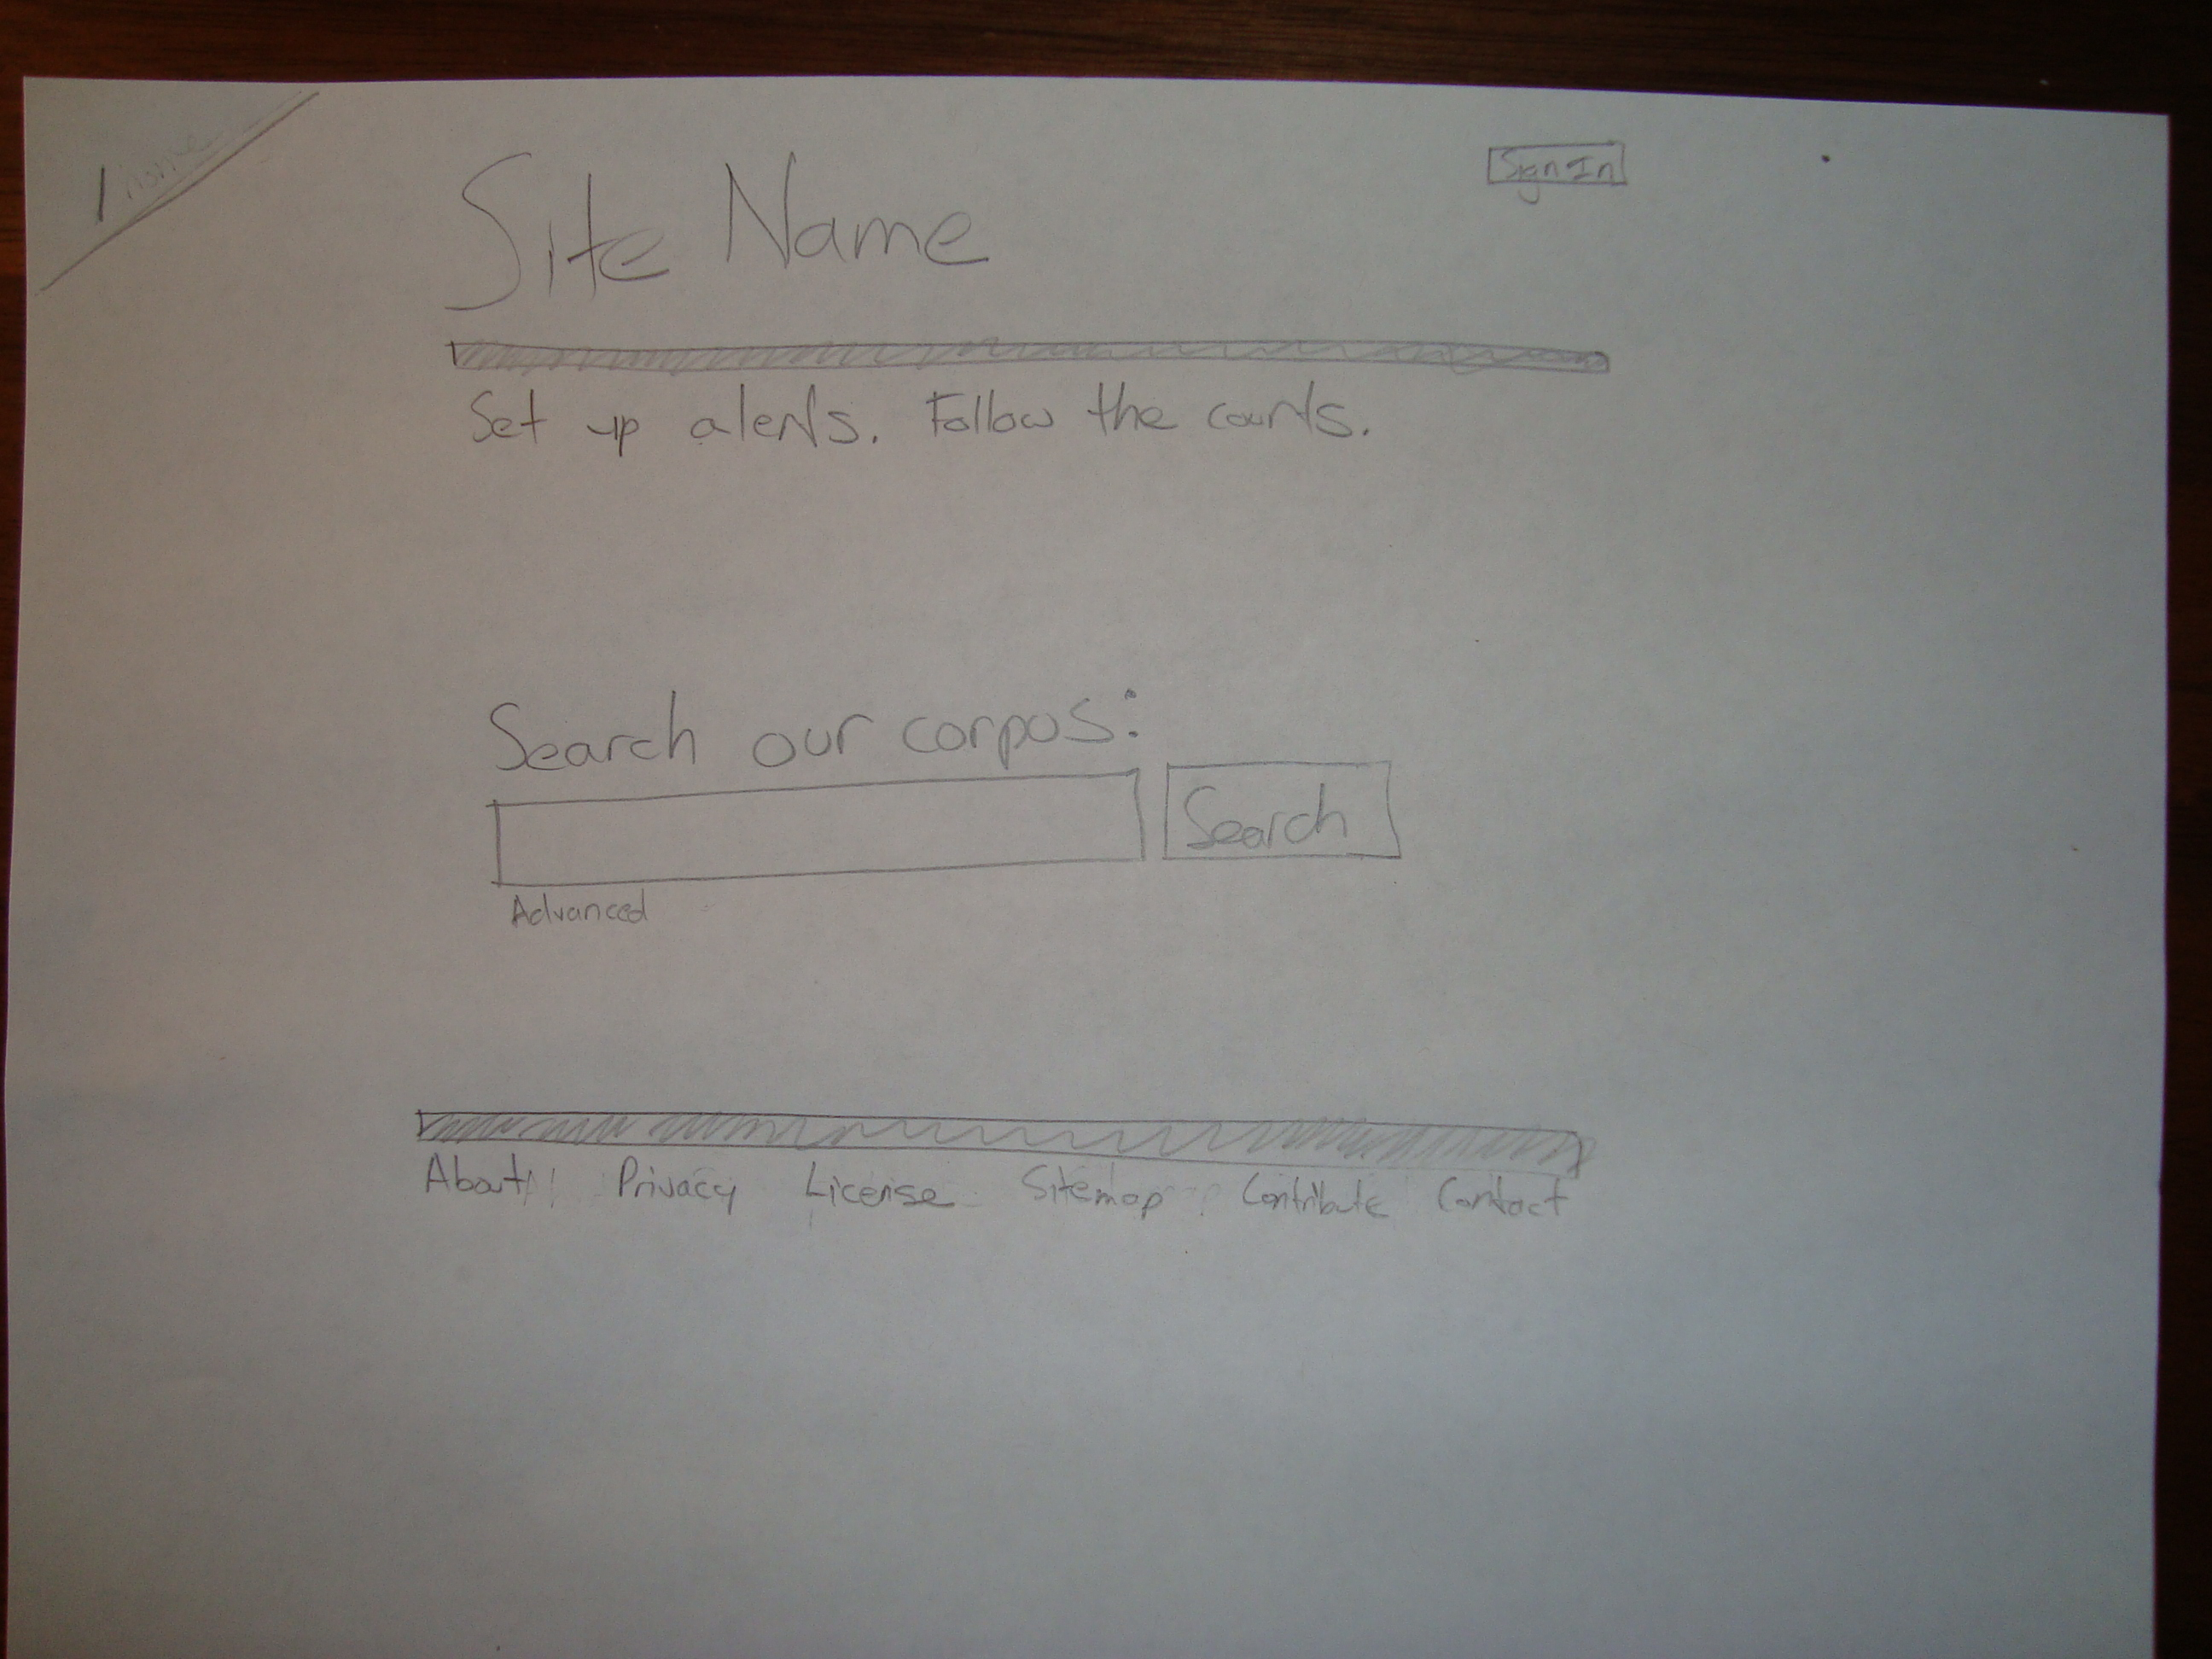
\includegraphics[width=0.85\textwidth]{DSC02180.JPG}

    \emph{Figure 1} --- The first sketch of the home page
    \vspace{5mm}

    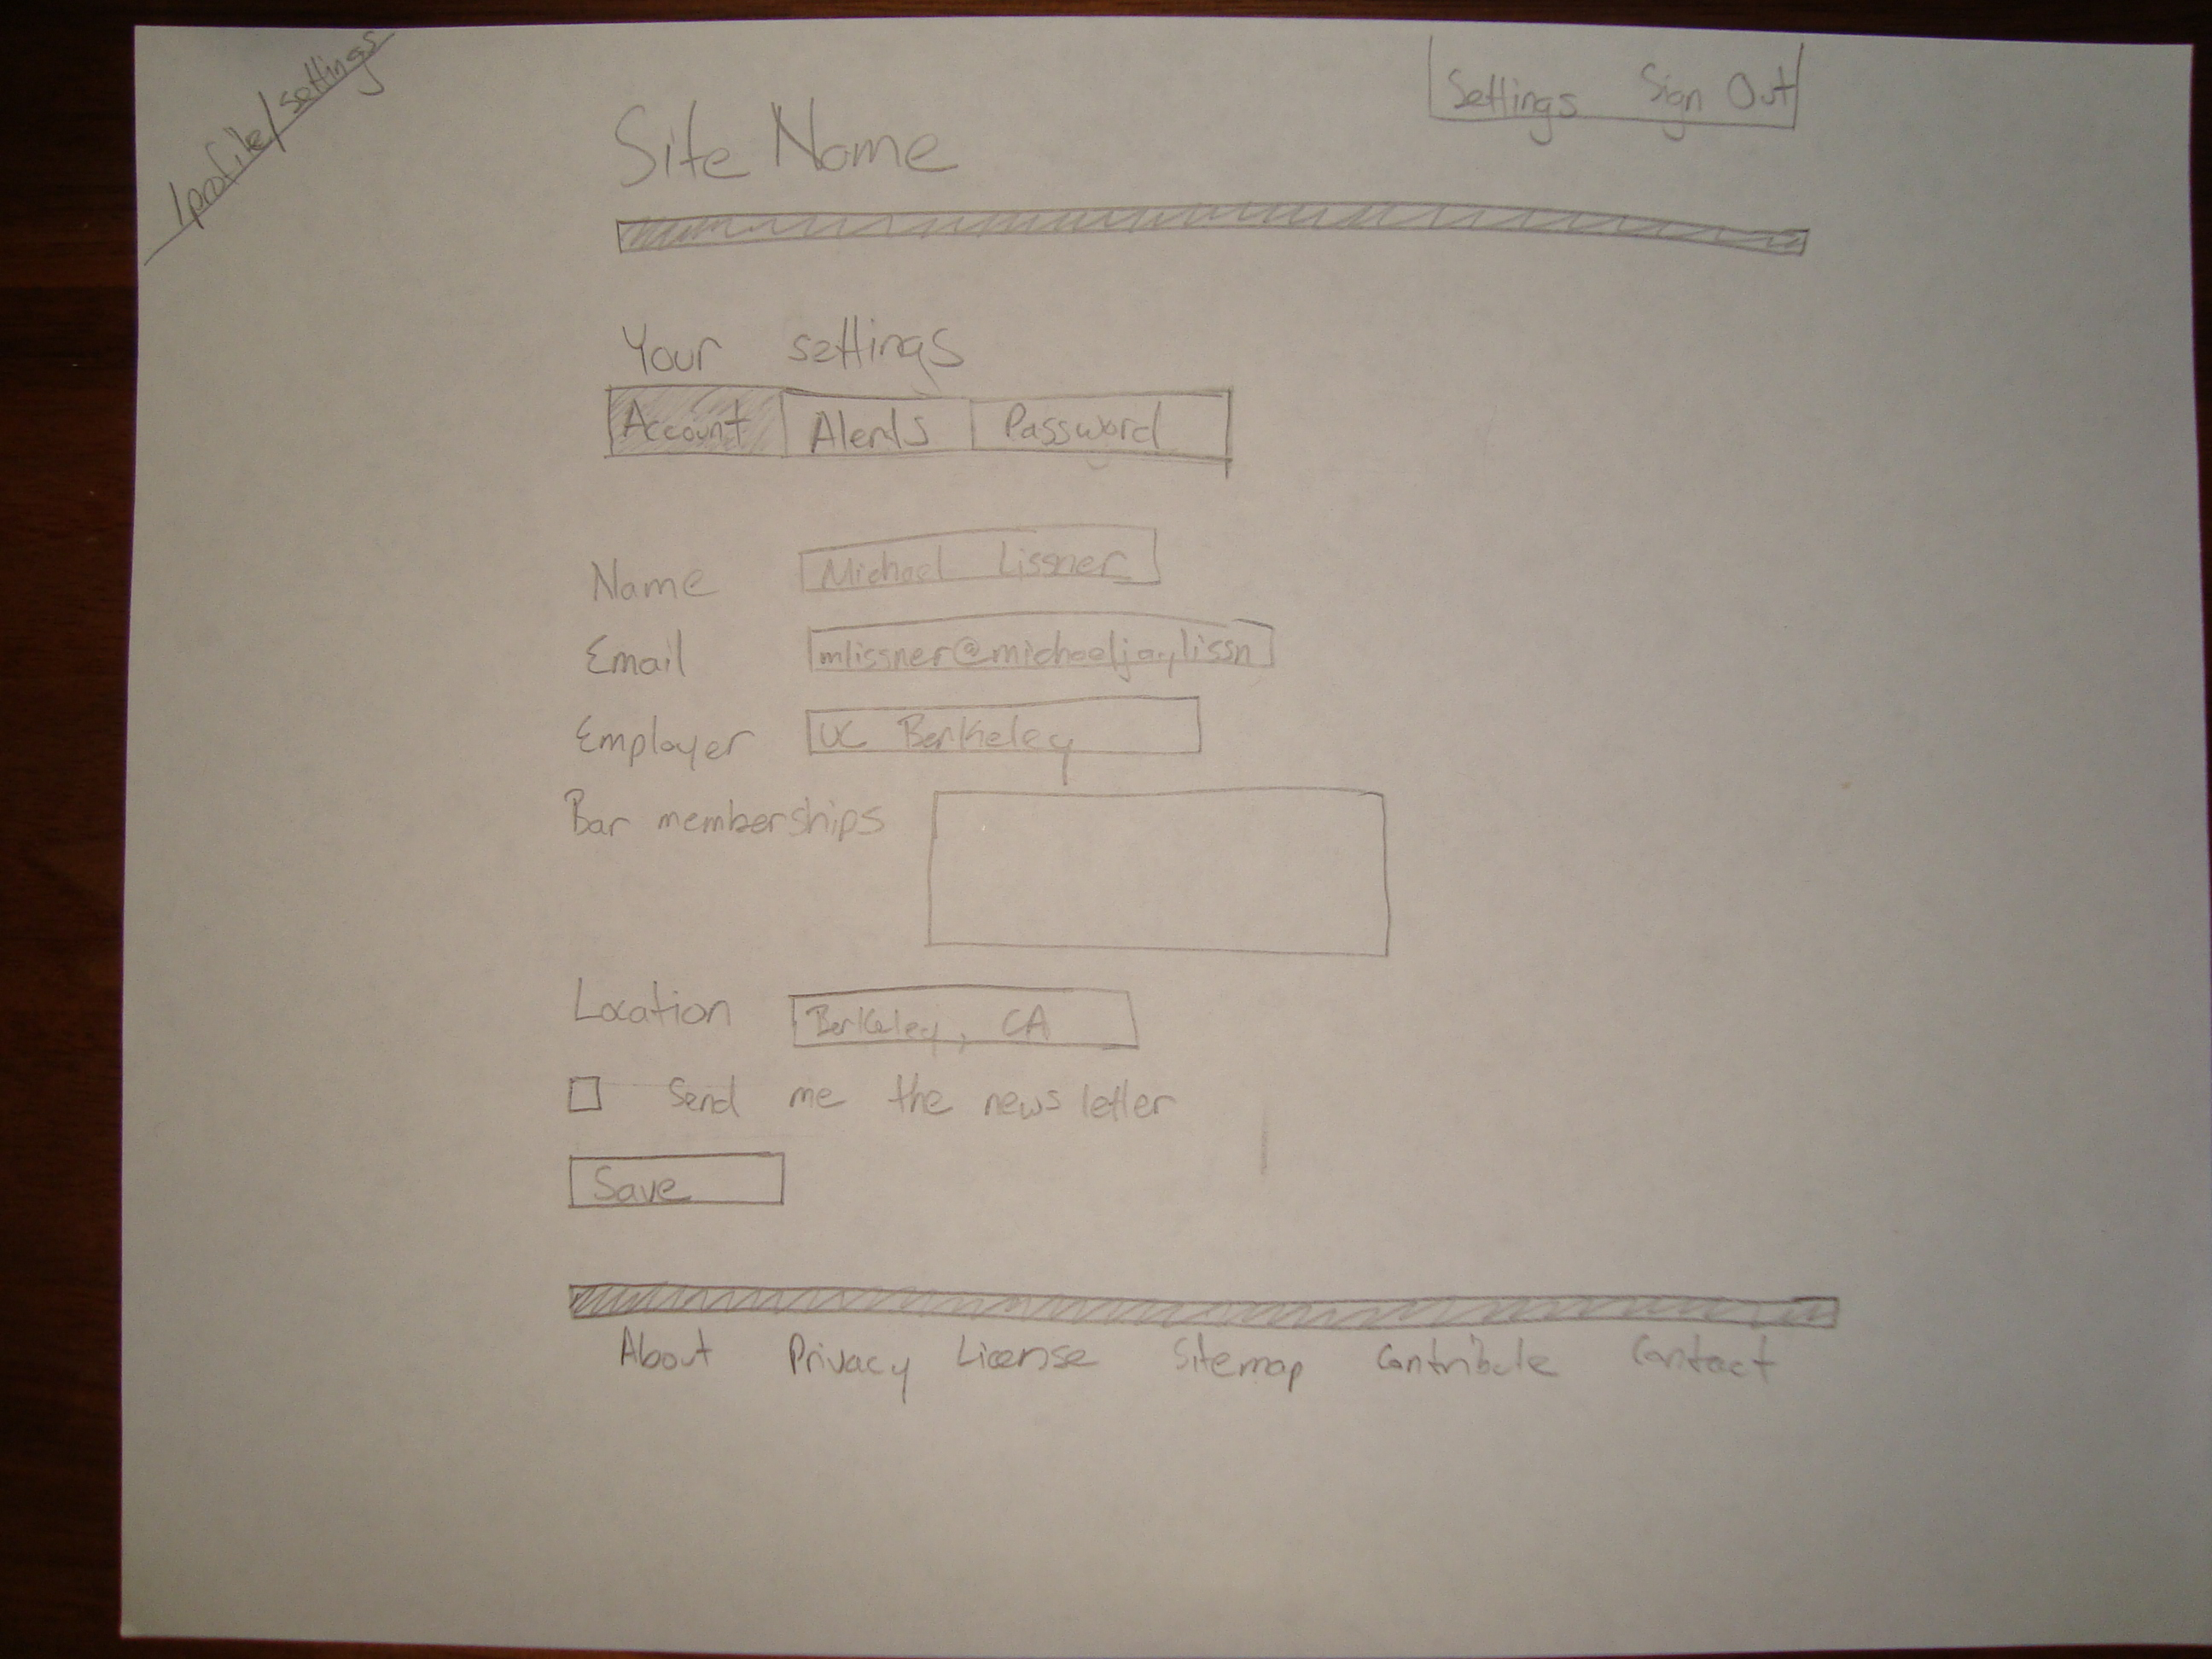
\includegraphics[width=0.85\textwidth]{DSC02184.JPG}

    \emph{Figure 2} --- The user profile page (/profile/settings/)
    \vspace{5mm}

    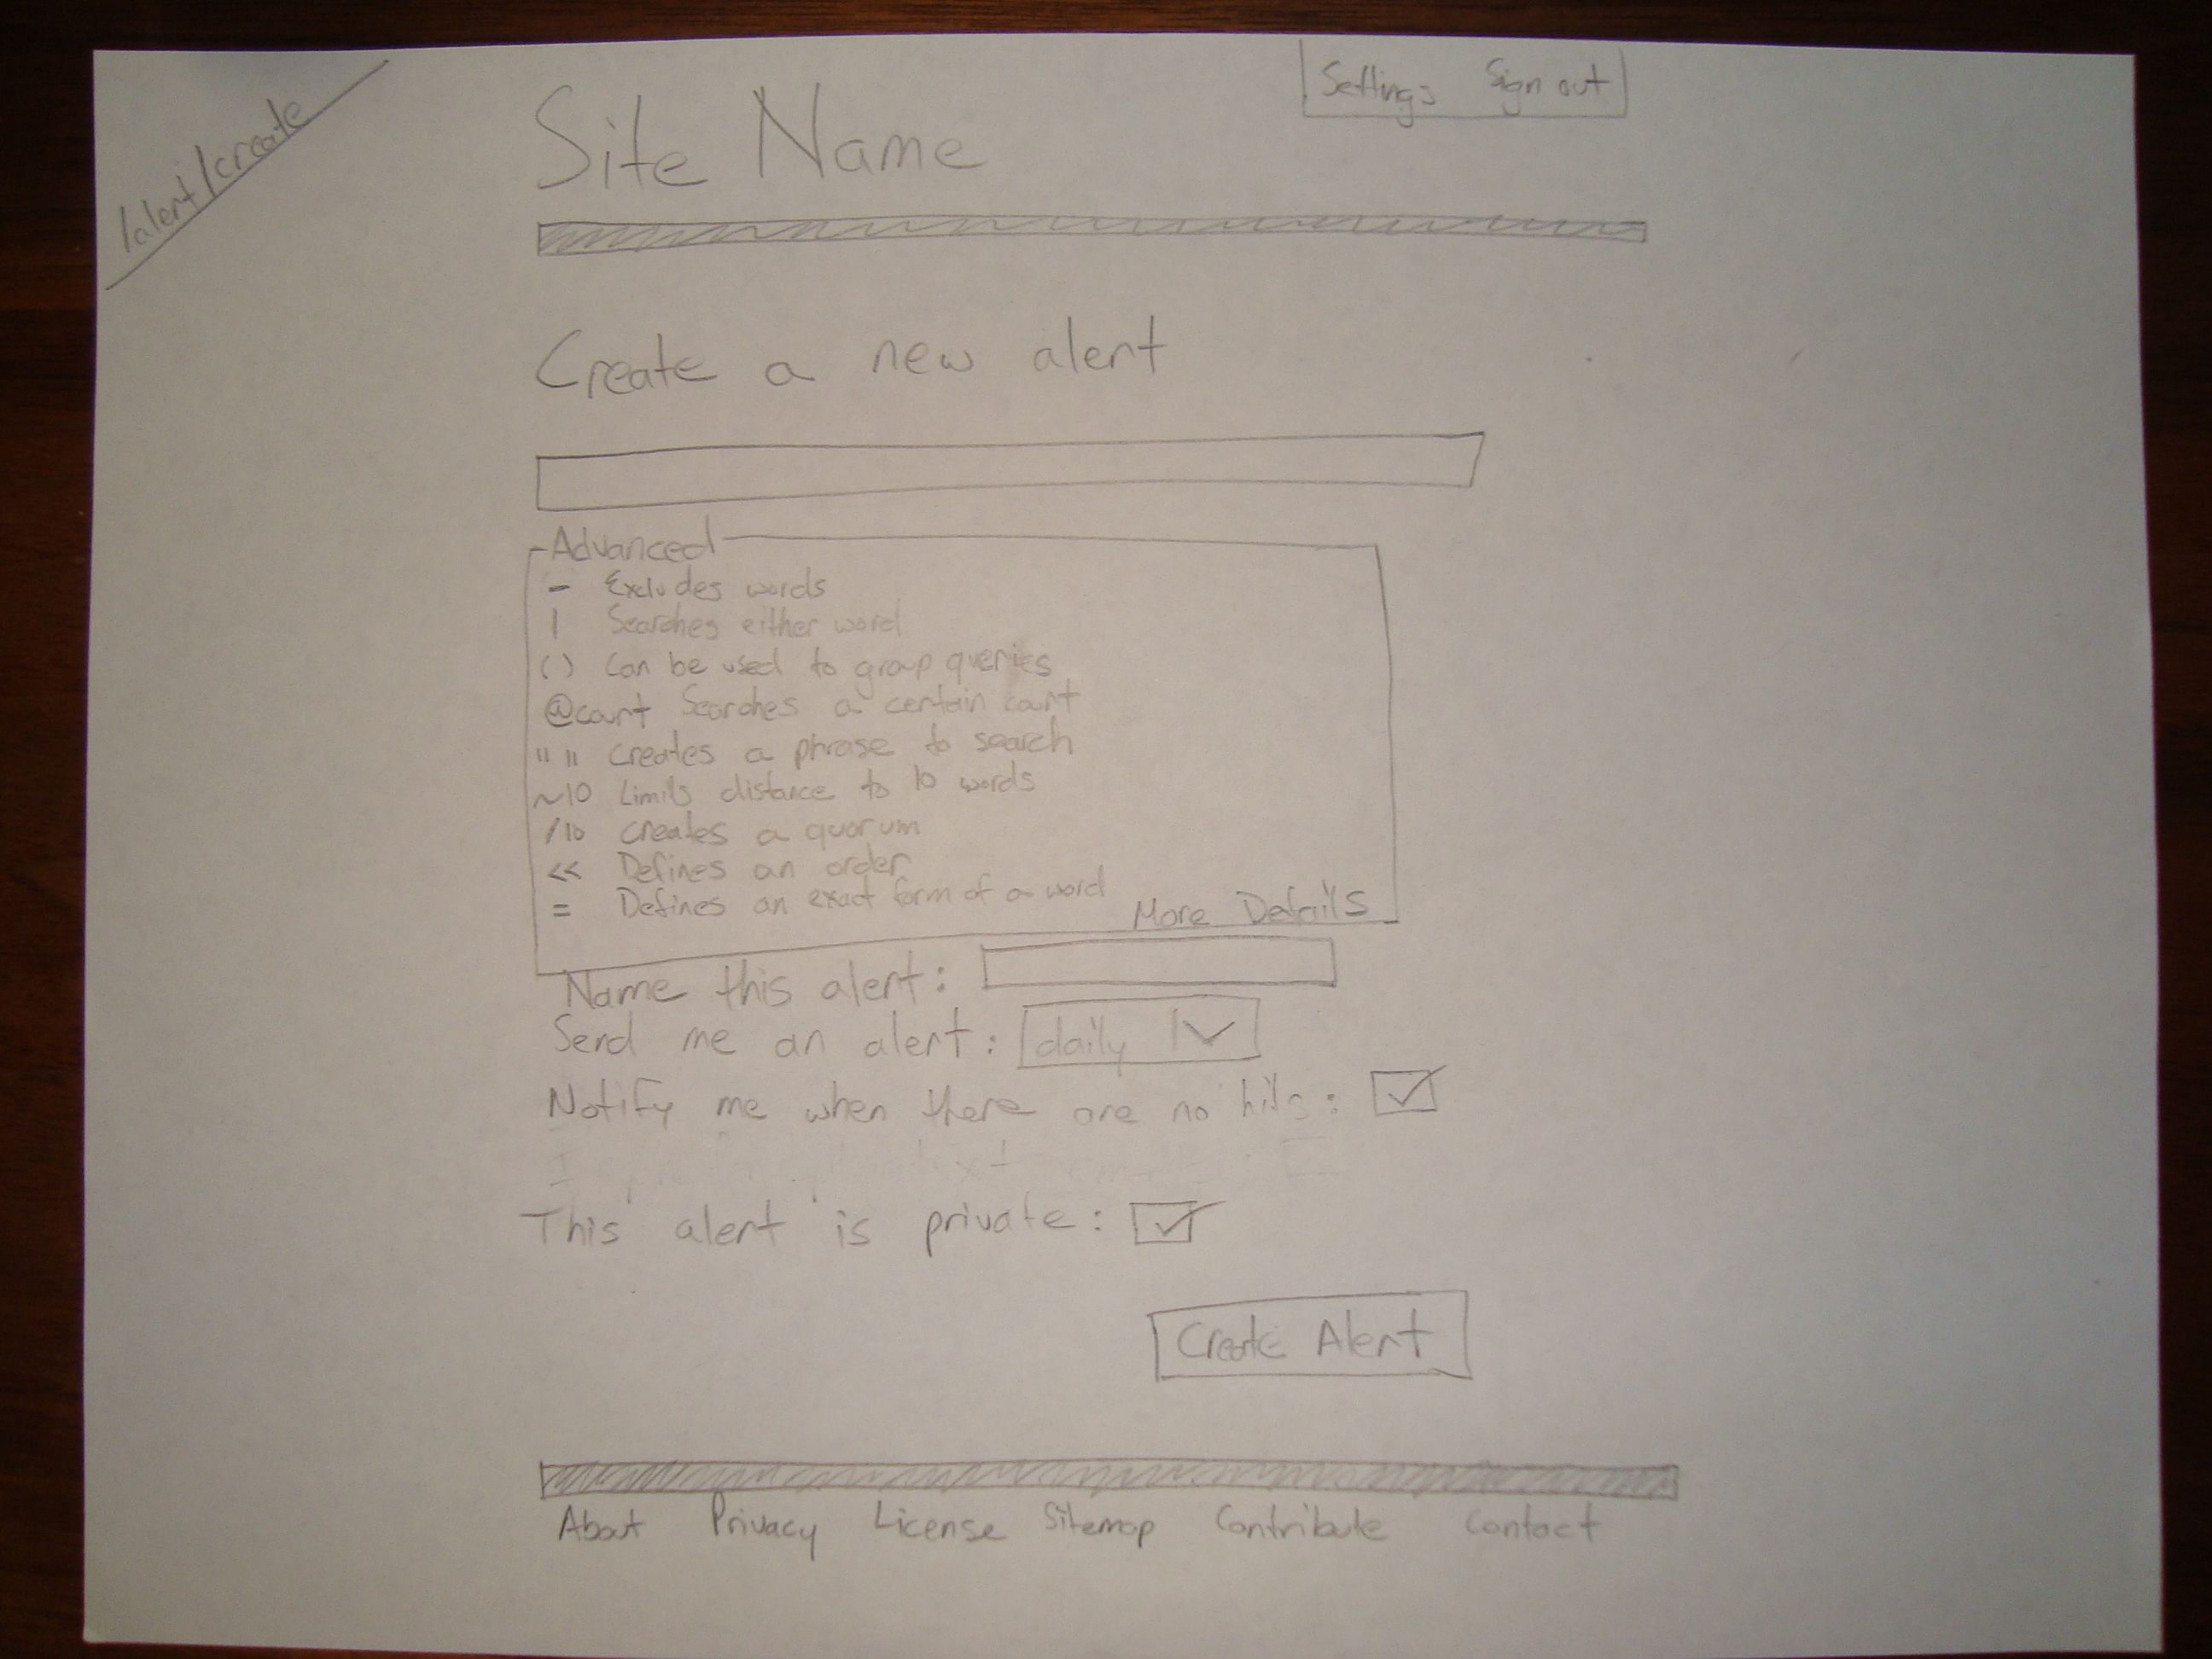
\includegraphics[width=0.85\textwidth]{DSC02183.JPG}

    \emph{Figure 3} --- The alert creation page (/alert/create/)
    \vspace{5mm}

    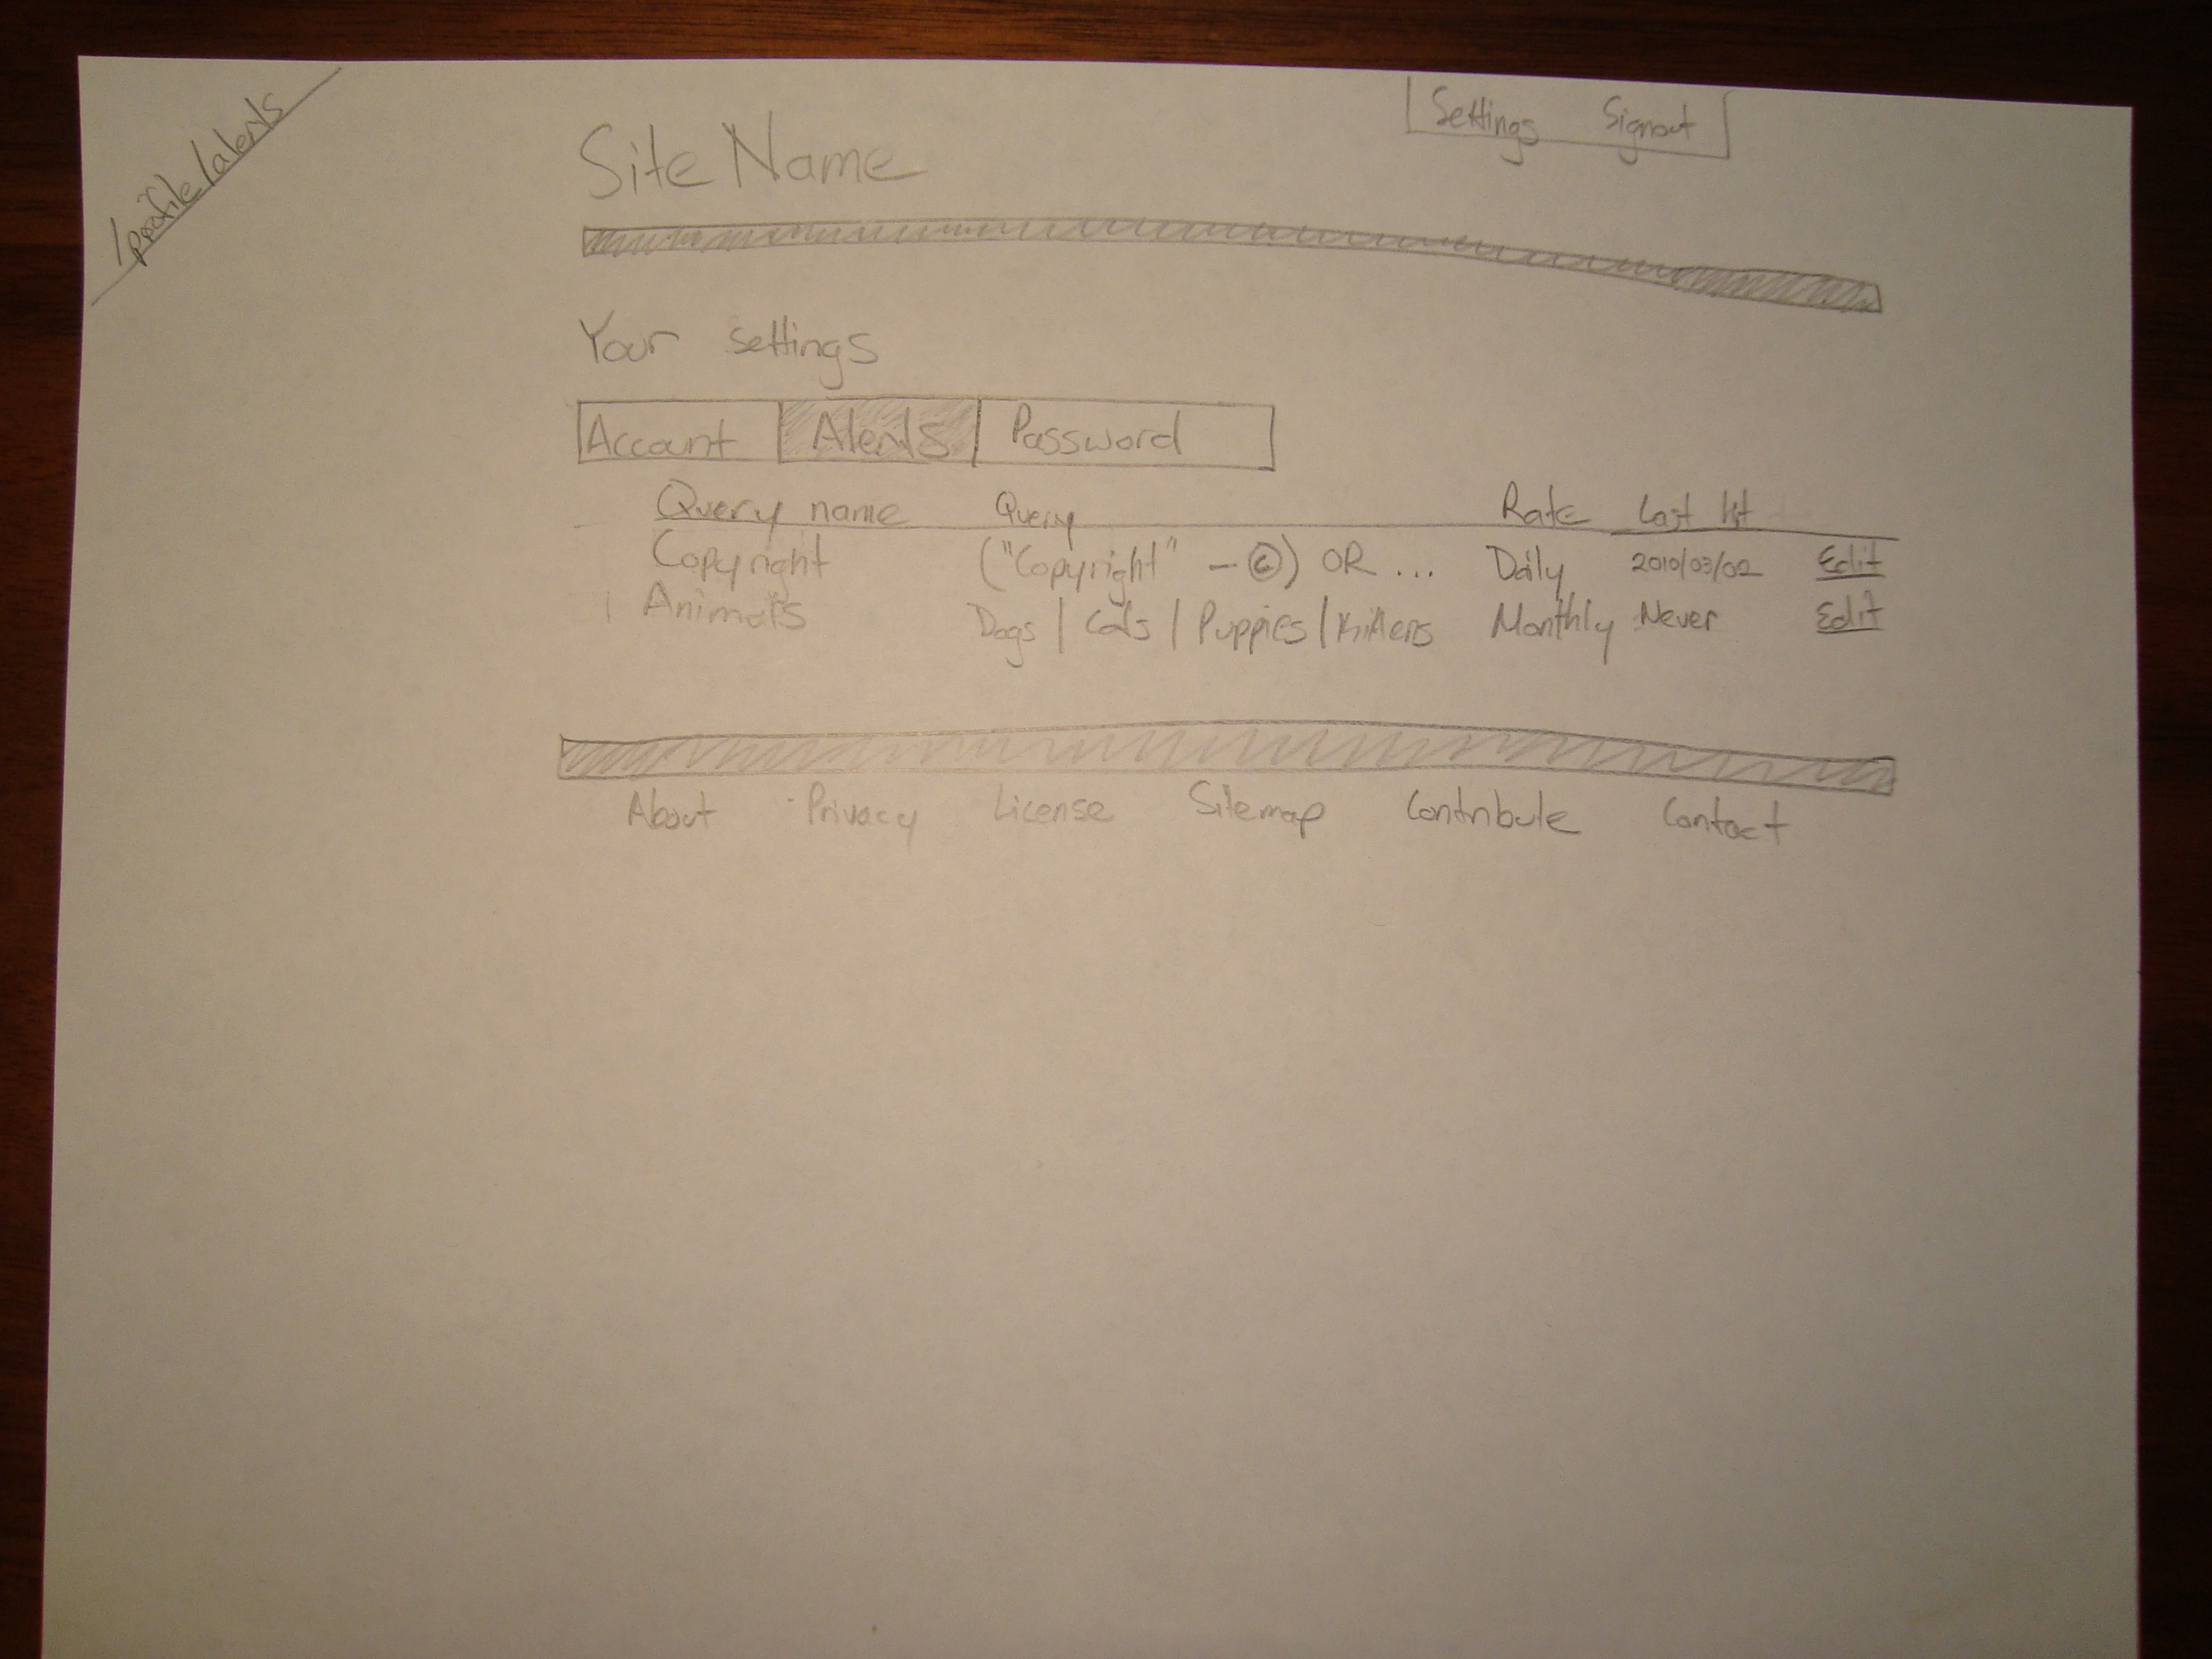
\includegraphics[width=0.85\textwidth]{DSC02185.JPG}

    \emph{Figure 4} --- The user alerts page (/profile/alerts/)
    \vspace{5mm}
\end{flushleft}


\clearpage
%\printbibliography UNCOMMENT THIS TO TURN THE BIBLIOGRAPHY BACK ON

% No longer necessary with biblatex package.
%\bibliographystyle{plain}
%\bibliography{bibliography}

\end{document}
